% Part 2 chapter following ch:electroweak. Carries "The Higgs Boson and the Origin of Duration: Electroweak Symmetry Breaking as the First
% Irreversible Act" (Mar 2026; book_sources_wave3.zip particle/iam_higgs_duration.tex, 746 lines, read in full 2026-10-02 for the first time).
% Physics wording replaces the source's philosophical vocabulary ("being/becoming", "duration", efficient cause, "Davar" are not carried).
% Corrections: PAPER_ERRATA HD1-HD12 (MANIFEST_particle.md); EW3-EW5 and TR8 apply. Numbers: docs/verification/scripts/verify_particle_book.py
% (H1-H10) and verify_entanglement_electroweak.py (W1-W12). Survey forecasts: Section sec:sp_euclid.
% Figure: docs/book/figscripts/fig_p2_particle.py (fig_higgs_proper).
\chapter{The Higgs field and the onset of proper time}\label{ch:higgsrecord}

\section*{The place}
Chapter~\ref{ch:electroweak} set out the particle physics of the electroweak crossover: which interactions bind, which symmetries the weak
interaction breaks, and when the crossover happens. This chapter reads that epoch as a record: the moment at which massive matter begins to accumulate proper time and the photon is fixed outside the
matter sector. It states what standard physics establishes, what IAM adds as interpretation, what the crossover sets and what is set elsewhere,
and what can be tested.

\section{What changes at the crossover}\label{sec:hr:change}
For the measured Higgs mass the Standard Model has no electroweak phase transition. Lattice studies find a smooth crossover~\cite{Kajantie1996},
centred at $T_c=159.5\pm1.5$\,GeV~\cite{DOnofrio2016}. \observed{} In the radiation era, $t=0.301\,g_*^{-1/2}\mP/T^2$ with $g_*=106.75$ puts it at
$t=9.2\times10^{-12}$\,s ($9.0$--$9.4\times10^{-12}$\,s across the quoted range of $T_c$). \calc{} Below the crossover the Higgs field takes its vacuum
value $v=(\sqrt2G_F)^{-1/2}=246.22$\,GeV~\cite{Englert1964,Higgs1964}. The particle that carries the field was found in 2012~\cite{ATLAS2012Higgs,CMS2012Higgs};
its mass is $m_H=125.20\pm0.11$\,GeV~\cite{PDG2024}, so the quartic coupling is $\lambda=m_H^2/2v^2=0.129$. \calc

The masses acquired are $M_W=80.3692\pm0.0133$\,GeV, $M_Z=91.1880\pm0.0020$\,GeV for the gauge bosons, and $m_f=y_fv/\sqrt2$ for the charged
fermions~\cite{PDG2024}. \observed{} The Yukawa couplings span almost six orders of magnitude, from $y_e=2.9\times10^{-6}$ to $y_t=0.991$. \calc{}
Each massive particle carries an internal clock, its Compton time $\hbar/mc^2$ (Table~\ref{tab:hr:masses}, Figure~\ref{fig:hr:proper}a). The
photon stays massless under the unbroken electromagnetic $U(1)$; the experimental bound is $m_\gamma<10^{-18}$\,eV~\cite{PDG2024}. \observed

\begin{table}[htbp]\centering\small
\caption{Rest masses acquired at the electroweak crossover and their Compton times. PDG 2024~\cite{PDG2024}; $v=246.22$\,GeV;
\texttt{verify\_particle\_book.py} (H2, H3).}\label{tab:hr:masses}
\begin{tabular}{lllll}\toprule
particle & mass (GeV) & coupling to the Higgs field & $\hbar/mc^2$ (s) & $m/T_c$\\\midrule
$e$ & $5.110\times10^{-4}$ & $y_e=2.94\times10^{-6}$ & $1.29\times10^{-21}$ & $3.2\times10^{-6}$\\
$\mu$ & $0.10566$ & $y_\mu=6.07\times10^{-4}$ & $6.23\times10^{-24}$ & $6.6\times10^{-4}$\\
$\tau$ & $1.77693$ & $y_\tau=1.02\times10^{-2}$ & $3.70\times10^{-25}$ & $0.011$\\
$W^\pm$ & $80.3692$ & gauge, $M_W=gv/2$ & $8.19\times10^{-27}$ & $0.50$\\
$Z^0$ & $91.1880$ & gauge & $7.22\times10^{-27}$ & $0.57$\\
$H$ & $125.20$ & $\lambda=0.129$ & $5.26\times10^{-27}$ & $0.78$\\
$t$ & $172.57$ & $y_t=0.991$ & $3.81\times10^{-27}$ & $1.08$\\
$\gamma$ & $<10^{-27}$ & none ($U(1)_{\rm em}$ unbroken) & --- & ---\\\bottomrule
\end{tabular}
\end{table}

\section{Proper time is the physical content}\label{sec:hr:proper}
A worldline's own duration is its proper time, $d\tau=dt\sqrt{1-v^2/c^2}$. A massless excitation moves on a null geodesic and accumulates none,
$\Delta\tau=0$. A massive one accumulates $\Delta\tau>0$. \derived{} Above the crossover the rest masses vanish. The particles of the plasma carry
thermal masses, a collective effect of the medium that vanishes in vacuum (Chapter~\ref{ch:electroweak}). Below it the $W$, $Z$, Higgs and charged
fermions have rest mass and their excitations move on timelike worldlines. \observed{} The matter-sector criterion of the framework is stated in
these terms: a degree of freedom decoheres gravitationally only if it accumulates proper time. Applied to the crossover it gives the epoch from
which a matter sector exists, with the photon held outside it by an exact gauge symmetry. \derived{} (given the criterion). This is the precise
content of the phrase ``origin of duration'': the onset of rest-mass proper time for the Standard Model particles. It is not the origin of time,
of entropy production or of irreversibility, all of which exist on both sides of the crossover.

\section{What the crossover sets, stated precisely}\label{sec:hr:corrections}
Each point below states exactly what belongs to the crossover and what belongs elsewhere.
\begin{enumerate}
\item \textbf{Chirality and CP are present on both sides of the crossover.} The gauge group $SU(2)_L\times U(1)_Y$ acts only on left-handed doublets at every
temperature, so parity violation is a property of the theory above the crossover as well as below. The CP-violating phase sits in the Yukawa
couplings, which are present on both sides; Jarlskog's invariant built from the quark mass matrices measures it~\cite{Jarlskog1985}. \observed{}
The crossover makes both visible in a massive spectrum. It does not establish them.
\item \textbf{The arrow of time holds for every interaction.} Entropy production, decoherence and Landauer's bound hold for every interaction
(Chapter~\ref{ch:electroweak}). Irreversible processes occur in the plasma before the crossover. \derived
\item \textbf{The strong interaction is virialised in the linear form, not the $1/r$ form.} The Cornell potential is linear at the confinement scale, where
$2\langle K\rangle=+\langle V_{\rm lin}\rangle$, not $2\langle K\rangle+\langle V\rangle=0$ (Chapter~\ref{ch:electroweak}). Of the three binding
interactions, only gravity and electrostatics have the virial half. \derived
\item \textbf{$E(a)$ is never zero.} Since $1-1/a=-z$, the activation function is $E=e^{-z}$. At the crossover $a=4.9\times10^{-16}$ and
$\ln E=-2.04\times10^{15}$: vanishingly small, not zero, and without a step at the crossover (Figure~\ref{fig:hr:proper}b). \calc{} $E=0.17$ falls
at $z=1.77$, a cosmic age of $3.67$\,Gyr (Planck 2018 $\Lambda$CDM, $H_0=67.36$, radiation included); at an age of $9$\,Gyr ($z=0.44$) $E=0.64$. \calc
\item \textbf{The baryon asymmetry needs more than the Standard Model crossover.} In the Standard Model the crossover cannot produce $\eta$: electroweak baryogenesis
needs a first-order transition and more CP violation than the quark mixing phase gives (Chapter~\ref{ch:electroweak}). The asymmetry may have
been set much earlier, for example through leptogenesis~\cite{FukugitaYanagida1986}. When $\eta$ was set is unknown. \observed
\item \textbf{The dark-matter density was in place at recombination.} The acoustic peaks of the microwave background fix the cold dark matter
density at $z\approx1090$: $\Omega_ch^2=0.120$~\cite{Planck2018VI}. The comoving density of dark matter was in place at recombination. \observed{} The
framework's identification of dark matter with the geometric half of the virial partition is a conjecture, and any version of it must reproduce
a dark-matter density already fixed at $z\approx1090$. \conjecture
\item \textbf{$\Omega_m/[\beta_mE(1)]=2$ is a definition.} With $\beta_m=\Omega_m/2$ and $E(1)=1$ the ratio is 2 identically. It is not a measured
virialisation of the universe. \derived
\item \textbf{The photon's masslessness and $\Sigma=1$ are separate statements.} Masslessness keeps photons on null geodesics and out of the matter sector. $\Sigma$
describes how the lensing potential $\Phi+\Psi$ responds to matter; weak lensing tests it (Chapter~\ref{ch:electroweak}). \derived
\item \textbf{The points of the Higgs vacuum are gauge-equivalent.} The points of the Higgs vacuum manifold are related by local gauge transformations. A local gauge
symmetry cannot break spontaneously~\cite{Elitzur1975}; the points are not distinct physical states, and no gauge-invariant quantity records which
one was taken. The gauge-invariant change across the crossover, the growth of $\langle\phi^\dagger\phi\rangle$, is smooth. \derived
\end{enumerate}

\section{The reading in IAM's terms}\label{sec:hr:reading}
The statement in IAM's terms is precise. IAM's Law prices records written by the matter sector at the temperature of the surface that receives
them. The crossover is the epoch from which the Standard Model supplies rest-mass worldlines that can write such records. On the framework's
criterion it is therefore the first epoch at which gravitational records by massive matter are possible. \interp{} It is not the first irreversible
event, and it is not the epoch at which those records are written in quantity: $E(z{=}30)=9.4\times10^{-14}$ and $E(z{=}10)=4.5\times10^{-5}$
(Chapter~\ref{ch:electroweak}). \calc

A further step would make the crossover itself a record: the field, in a superposition over its vacuum manifold, decoheres into one vacuum and pays
the Landauer price at $T_c$, $\kB T_c\ln2=110.6$\,GeV per bit. \calc{} By Section~\ref{sec:hr:corrections}, item~9, the Standard Model crossover has no gauge-invariant outcome to record, so the step is carried in its
open form. \conjecture{} The open form of the question is whether any physical outcome is selected at the electroweak epoch. \openprob

\begin{figure}[htbp]\centering
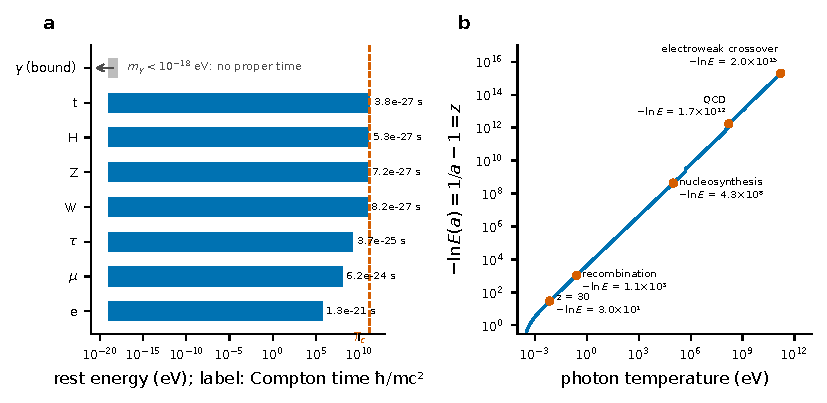
\includegraphics[width=\textwidth]{figures/part2/fig_higgs_proper.pdf}
\caption[Masses, clocks and the activation function across the crossover]{(a) Rest energies acquired at the electroweak crossover (PDG
2024~\cite{PDG2024}) with each particle's Compton time $\hbar/mc^2$; the dashed line is $T_c=159.5$\,GeV~\cite{DOnofrio2016}. The photon bound,
$m_\gamma<10^{-18}$\,eV, leaves it without proper time. (b) $-\ln E(a)=1/a-1=z$ against the photon temperature, from the crossover
($2.0\times10^{15}$) through QCD confinement, nucleosynthesis and recombination ($1.1\times10^3$) to $z=30$; $a(T)$ from entropy conservation with
a step approximation of $g_{*s}(T)$, $g_{*s}=3.938$ today. $E(a)$ has no step at the crossover. \calc}\label{fig:hr:proper}
\end{figure}

\section{Testable content}\label{sec:hr:tests}
\begin{enumerate}
\item \textbf{The Standard Model crossover.} It leaves no gauge-invariant record, and so the reading predicts nothing that a measurement of the
crossover could check. \openprob
\item \textbf{A first-order transition.} Extensions of the Standard Model can make the electroweak transition first order. Bubbles of the broken
phase are then distinct physical outcomes, and their collisions source a stochastic gravitational-wave background~\cite{Caprini2016}. The Hubble
frequency at $T_c$, redshifted to today, is $2.7\times10^{-5}$\,Hz; the signal peaks higher by a factor of order $\beta/H$, the ratio of the transition rate to the
expansion rate (about $0.23\,\beta/H$ for bubble collisions and $1.15\,\beta/H$ for sound waves at wall speed $c$~\cite{Caprini2016}): of order $10^{-4}$--$10^{-2}$\,Hz for $\beta/H=10$--$1000$, the band of a space interferometer. \calc{} A detection would turn the open
question of Section~\ref{sec:hr:reading} into a question about measured outcomes. A null result would not decide it. \openprob
\item \textbf{The sector split.} The reading inherits the framework's two late-time tests (Chapter~\ref{ch:electroweak}). $\Sigma=1$ at every
redshift is tested by tomographic weak lensing; a significant $\Sigma\neq1$ falsifies the photon exemption. \prediction{} For $\mu$, the
forecast with IAM's own $\mu(z)$ is in Section~\ref{sec:sp_euclid}.
\item \textbf{The baryon asymmetry.} A revised $\eta$ would revise $\Omega_b$ and the baryonic part of $\beta_m=\Omega_m/2$. That is bookkeeping
inside a definition, not a test. \derived
\end{enumerate}

The electroweak epoch is where matter first carries its own clocks, and that alone makes it worth a closer look. A particle physicist can take the first-order question to the gravitational-wave band, and a cosmologist can take IAM's own $\mu(z)$ to the turn-on of the growth ramp.

\section{Status}\label{sec:hr:status}
\begin{center}\small\begin{tabularx}{\linewidth}{@{}>{\raggedright\arraybackslash}X>{\raggedright\arraybackslash}p{0.3\linewidth}@{}}\toprule
statement & label\\\midrule
crossover at $T_c=159.5\pm1.5$\,GeV, $t=9.2\times10^{-12}$\,s; $v=246.22$\,GeV; $m_H=125.20$\,GeV & \observed{} / \calc\\
rest masses and proper time below the crossover; photon massless & \observed\\
the matter sector exists from the crossover & \derived{} (given the criterion)\\
the crossover as the first epoch at which massive matter can write gravitational records & \interp\\
chirality, CP violation, the arrow of time and $\eta$ are not created at the crossover & \observed\\
$E=e^{-z}$, never zero; $\ln E(a_{\rm EW})=-2.04\times10^{15}$ & \calc\\
dark-matter density fixed by $z\approx1090$ & \observed\\
the vacuum ``choice'' as a record & \conjecture{} (open form only: Elitzur)\\
whether any physical outcome is selected at the electroweak epoch & \openprob\\
$\Sigma=1$; $\mu_0=-0.136$ (forecast: Section~\ref{sec:sp_euclid}) & \prediction\\\bottomrule
\end{tabularx}\end{center}
